\documentclass[12pt]{article}

\usepackage[T3]{fontenc}
\usepackage[utf8]{inputenc}
\usepackage[russian]{babel}

\usepackage{graphicx}
\usepackage{mhchem}

\usepackage{gensymb} % degree symbol
\usepackage{nicefrac} % nice fractions
\usepackage{mathtext}

\usepackage{titling}

\title{Определение удельной энтальпии растворения неорганической соли в \ce{H2O}}
\date{}

\newcommand{\tn}{\textnormal}
\newcommand{\vlevo}{\hspace*{-0.63cm}}

\setlength{\droptitle}{-10em}

\begin{document}

\maketitle

\vspace*{-3cm}

В калориметрическую систему было помещено $m = 24.31 \tn{г.}$ $\ce{KCl}$.  
Было проведено 20 замеров температуры с интервалом в 30 секунд, из которых 8 было сделано до добавления соли, а 12 -- после добавления. \\
Теплоемкость используемой калориметрической системы: $W = 2090 \ \nicefrac{ \tn{кал.}}{{}^{\circ}C}$.

\vlevo Полученная температурная зависимость имеет следующий вид:

\begin{figure}[!h]
  \centering
	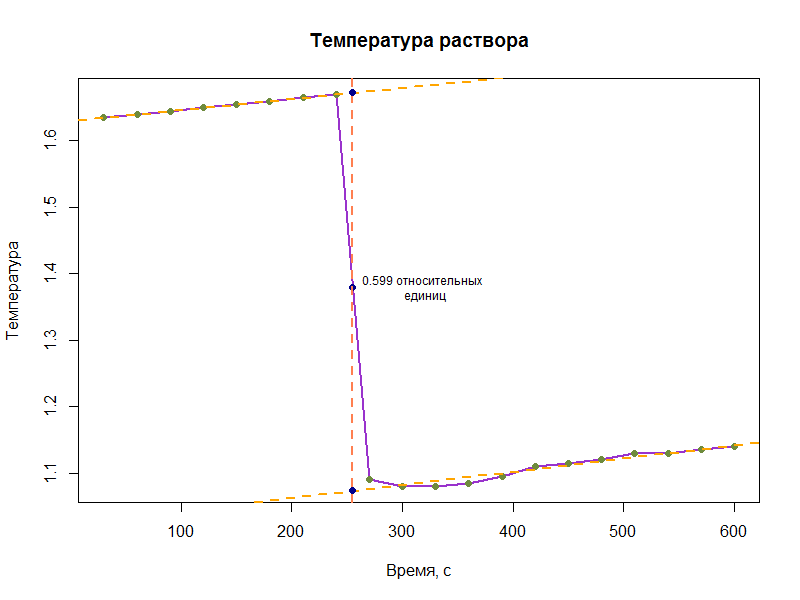
\includegraphics[width=0.7\textwidth]{Rplot.png}
	\caption{График температурной зависимости.}
	\label{fig:Temperature}
\end{figure}

Учет температурных поправок производился графическим способом. Группы точек до скачка и после были аппрокисимированы линейными зависимостями. Величина скачка определяется разностью между ординатами точек, полученными пересечением вертикальной прямой, проведенной через середину проекции скачка на ось абсцисс, с двумя прямыми, аппроксимирующими изменение температуры до скачка и после.
Полученное значение температурного скачка: \( \Delta t = 0.699^{\circ}C\)

Значение энтальпии растворения вычислялось по следующей формуле:
\( \Delta H_{\tn{раств.}} = \nicefrac{W \Delta t}{m} = 16.14 \, \nicefrac{\tn{кДж}}{\tn{моль}}\) \\
Представленное в литературе значение энтальпии растворения:
\( \Delta H_{\tn{раств.}}^{\tn{лит.}} = 17.00 \, \nicefrac{\tn{кДж}}{\tn{моль}} \)

\end{document}